\subsection{Éléments d'identification du \emph{Particle Flow}}\label{chapter-LHC-section-evt_reco-subsec-PF_elements}
\subsubsection{Traces des particules chargées et vertex}
Les particules chargées laissent des traces de leur passage dans le trajectographe et, dans le cas des muons, dans les chambres à muons.
La structure du trajectographe présentée en section~\ref{chapter-LHC-section-CMS-subsec-tracker} ne donne pas de traces continues mais des points de passage de ces particules.
\par Les traces des particules sont alors reconstruites à partir de ces points de passage à l'aide d'une méthode itérative~\cite{track_reco}.
Les traces présentant au moins huit points de passage avec au plus un point manquant le long de l'extrapolation obtenue sont considérées pour la suite de la reconstruction~\cite{particle-flow}.
Il est également requis que les traces proviennent d'un cylindre de quelques millimètres de rayon autour du faisceau et qu'elles correspondent à une impulsion transverse minimale de \SI{0.9}{\GeV}.
Les performances de cette méthode sont discutées dans la référence~\cite{CMS_TDR_1}.
\par La combinaison de ces traces permet de reconstruire les vertex d'interactions de l'événement.
Plusieurs vertex sont présents du fait de l'empilement.
Le vertex principal est choisi comme étant le vertex dont la somme des impulsions transverses au carré des traces en provenant est la plus élevée, les autres sont considérés comme des vertex de l'empilement.
L'efficacité de reconstruction du vertex principal est ainsi de l'ordre de \SI{100}{\%}, celle des vertex de l'empilement de \SI{70}{\%}~\cite{JERC_RunI}.
\par Les particules peuvent être déviées par interaction avec la matière du trajectographe~\cite{moliere_scat_1,moliere_scat_2}.
Un algorithme dédié à ce phénomène est utilisé et permet de déterminer les lieux de ces interactions, représentés sur la figure~\ref{fig-chapter-LHC-section-evt_reco-subsec-PF_elements-CMS-self-radio}.
La structure du trajectographe se retrouve et le taux de mauvaise reconstruction est réduit par un traitement spécifique des traces présentant de telles déviations.
\begin{figure}[h]
\centering
\subcaptionbox{Dans le plan longitudinal \plane{r}{z}.\label{subfig-chapter-LHC-section-evt_reco-subsec-PF_elements-particle-flow-Figure_005-a}}[.45\textwidth]
{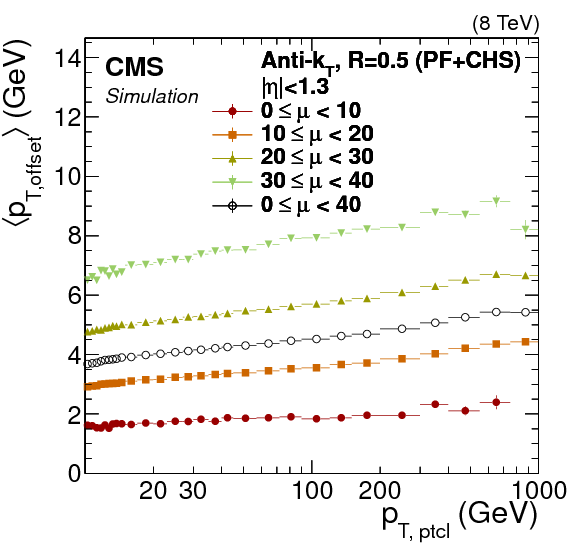
\includegraphics[width=.45\textwidth]{\PhDthesisdir/plots_and_images/from_particle-flow/Figure_005-a.png}}
\hfill
\subcaptionbox{Dans le plan transverse \plane{x}{y}.\label{subfig-chapter-LHC-section-evt_reco-subsec-PF_elements-particle-flow-Figure_005-b}}[.45\textwidth]
{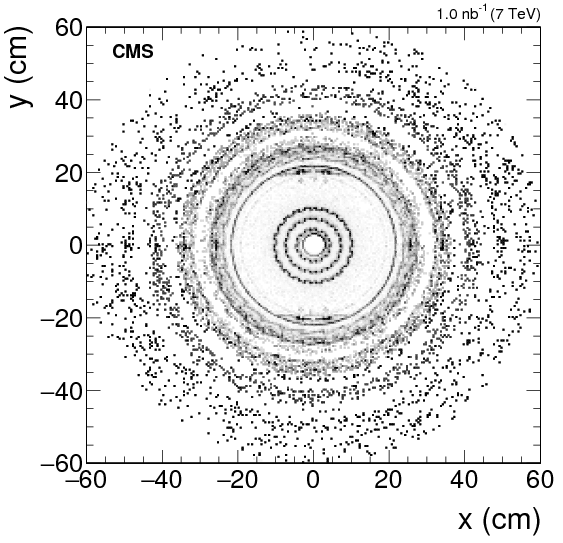
\includegraphics[width=.45\textwidth]{\PhDthesisdir/plots_and_images/from_particle-flow/Figure_005-b.png}}
\caption[Points d'interactions entre particules des événements et matière composant le détecteur.]{Carte des points d'interactions entre particules des événements et matière composant le détecteur~\cite{particle-flow} à partir de données prises en 2011 à $\sqrt{s}=\SI{13}{\TeV}$.}
\label{fig-chapter-LHC-section-evt_reco-subsec-PF_elements-CMS-self-radio}
\end{figure}
\par Les traces des électrons et des muons présentent des spécificités particulières.
Les électrons émettent avant de parvenir au ECAL une fraction non négligeable de leur énergie par \emph{bremsstrahlung}, \ie\ sous forme de photons.
Les performances de reconstruction des électrons dépendent ainsi fortement de la capacité à identifier ces photons et mesurer leurs énergies.
Dans le cas des muons, les signaux de leur passage dans le trajectographe et dans les chambres à muons permettent de définir trois types de traces pour les éléments de reconstruction:
\begin{itemize}
\item les muons seuls (\emph{standalone muons}), reconstruits uniquement à partir des signaux des chambres à muons;
\item les muons globaux (\emph{global muons}), obtenus par la correspondance d'une trace dans le trajectographe avec l'extrapolation de la trace d'un muon seul;
\item les muons du trajectographe (\emph{tracker muons}) sont les traces du trajectographe d'impulsion transverse supérieure à \SI{0.5}{\GeV} dont l'extrapolation passe par une des chambres à muons ayant détecté le passage d'une particule.
\end{itemize}
Plus de détails sont disponibles dans les sections~3.2 et~3.3 de la référence~\cite{particle-flow}.
\subsubsection{Dépôts dans les calorimètres}
Les dépôts dans les calorimètres sont regroupés de proche en proche en agglomérats (\emph{clusters})~\cite{particle-flow}, indépendamment pour chaque sous-partie des calorimètres.
Plusieurs raisons existent à cette agglomération:
\begin{itemize}
\item détecter et mesurer les énergies et directions des particules neutres stables comme les photons et les hadrons neutres;
\item séparer les dépôts des particules neutres de ceux des particules chargées;
\item reconstruire et identifier les électrons et les photons issus du \emph{bremsstrahlung} correspondant;
\item améliorer la mesure de l'énergie des hadrons chargés dont les traces sont imprécises.
\end{itemize}
\par La construction de ces agglomérats commence par l'identification des cellules des calorimètres mesurant une énergie supérieure à un seuil, défini pour chaque sous-partie des calorimètres.
Les cellules adjacentes sont ajoutées à l'agglomérat.
Puis, toute cellule avec au moins un coin en commun avec une cellule déjà dans l'agglomérat et mesurant une énergie supérieure à deux fois le niveau moyen du bruit est ajoutée à l'agglomérat.
\par Les photons et les hadrons neutres ne peuvent être reconstruits qu'à l'aide de leurs dépôts dans les calorimètres.
Des dépôts isolés vis-à-vis des traces de particules chargées sont ainsi une signature claire des particules neutres.
Cependant, un dépôt de particule neutre situé au même endroit qu'un dépôt de particule chargée est identifié comme un excès d'énergie par rapport à l'énergie déterminée à l'aide du trajectographe.
Les agglomérats obtenus sont alors calibrés afin de pouvoir identifier les dépôts de particules neutres chevauchant un dépôt de particule chargée.
Plus de détails sont disponibles dans la section~3.5 de la référence~\cite{particle-flow}.